
Computer vision is a field of artificial intelligence concerned with extracting information that is meaningful and useful to humans from digitised visual material (photos, videos) and then making decisions based on that information, using computers. Where artificial intelligence gives computers the ability to think, computer vision gives them the ability to see, observe, and understand their surroundings.

Computer vision functions similarly to human vision, but humans have a lifetime head start at this skill -- they begin learning to distinguish objects from birth. Over a lifetime a person becomes able to distinguish many objects, judge their distance, recognise whether they are stationary or moving, and detect defects in images or objects.

In computer vision, computers are ``trained'' to carry out similar operations, but much faster, using cameras, massive datasets, and algorithms in place of the human eye's retina, optic nerves, and the brain's visual interpretation. Such a system also has advantages over human vision, chiefly specialisation. Once we teach the system what a vessel and a buoy look like, the resulting detection model is able to analyse many hundreds of objects and situations per second and react with far greater accuracy, reliability, and speed than a human performing the same task.

Computer vision is in use in several fields: energy management (consumption forecasts), manufacturing (product-defect inspection), and the automotive industry (autonomous vehicles and driver-assistance systems), and the demand for computer vision specialists is on the rise \cite{ref14}.

\section{Computer vision operating principle}\label{computer-vision-operating-principle}

To train and create a computer vision model, a massive dataset is required; it is analysed many thousands of times until the model finds regularities, patterns, and -- in the case of objects -- characteristic shapes in the data, which finally allow it to identify the sought object independently in new, previously unseen images.

Machine learning is used to perform this task; it includes artificial neural networks and, within those, deep learning and convolutional neural networks in particular.

Machine learning uses algorithmic models that enable a computer to understand the content of visual data. Given a sufficient amount of data, the computer can teach itself, on the basis of that data, what an image contains and how images differ from one another. Algorithms enable the machine to learn on its own, which is significantly more efficient than a human pre-programming the computer to recognise images.

A convolutional artificial neural network helps the computer vision model understand an image by examining the input as several smaller, labelled regions. Convolutional operations are performed on the labelled regions, on the basis of which the neural network makes predictions about what it sees. The neural network repeats these operations and iteratively checks the accuracy of its predictions until the results are accurate enough and true. Once such an operation is successfully completed, the model is able to see and recognise images in a format understandable to a human \cite{ref14}.

\section{Convolutional neural network}\label{convolutional-neural-network}

The convolutional neural network (\emph{Convolutional Neural Network, ConvNet, CNN}) is a deep-learning algorithm that can find characteristic features of a given input image and distinguish them from one another. Compared with other image-recognition algorithms, the amount of preprocessing required for a CNN is significantly smaller. A CNN is also capable of creating filters on its own, with enough training, in order to distinguish image features (learning the peculiarities of images), unlike manually tuned algorithms, which cannot do this as accurately \cite{ref15}.

This neural network is distinguished from others by the layers that form its foundation:

\begin{itemize}
\item
  Convolutional layer
\item
  Pooling layer
\item
  Fully connected layer
\end{itemize}

The convolutional layer is the CNN's first layer, the fully connected layer is the last, and pooling and additional layers sit between them. With each successive layer the complexity of the network grows and the system's understanding of the input image becomes more complete. The upper layers grasp simpler features such as colours and edges. In deeper layers the system develops a more generalised understanding of the elements or images in the picture, and on the basis of the information obtained -- provided there is enough of it -- decides what the photo depicts.

The \textbf{convolutional} layer (\emph{convolutional layer}) is the most important part of a CNN; the largest amount of computation takes place here. This layer requires input data, a filter, and a feature map. Assume the input is a colour image in the form of a three-dimensional matrix (green, red, blue -- three channels; height, width, depth -- three dimensions). With that, the input data are defined. We also need a feature-detection function -- the kernel or \textbf{filter} -- which moves stepwise across the data, checks whether a particular feature is present in the image, and performs the corresponding computations. The operation just described is convolution.

The \textbf{filter} is a two-dimensional matrix filled with constant weights that represents a portion of the image. Filters come in various sizes, but traditionally they are three-by-three matrices. The filter is applied to a portion of the image, producing the dot product of the image region matrix and the filter matrix, which is passed on to the output matrix. The filter matrix then shifts forward by a predetermined number of pixels until this operation has been performed across the entire image, resulting in a map of convolutional features (see Figure 2.2.1).

\begin{figure}
\centering
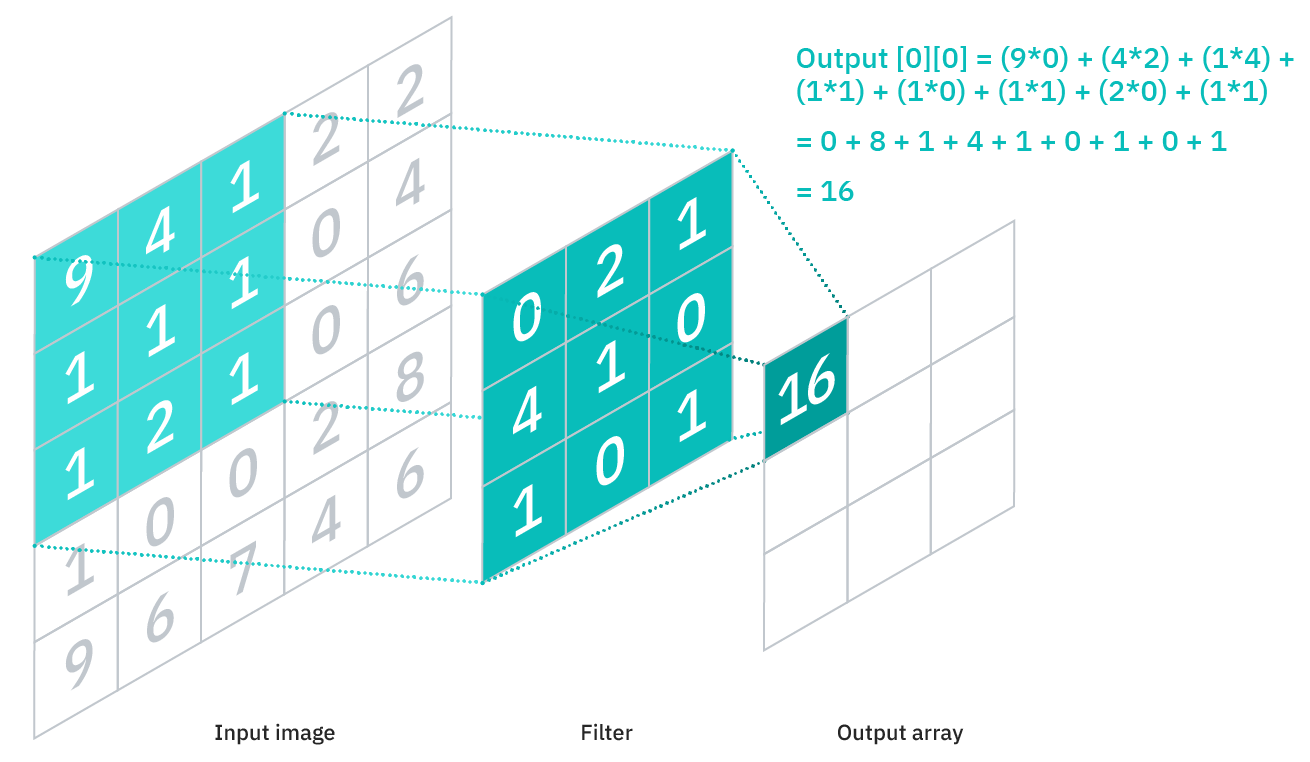
\includegraphics[width=6.10174in,height=3.55556in,alt={matrix multiplication in convolutional neural networks}]{media/image5.png}
\caption{matrix multiplication in convolutional neural networks}
\end{figure}

Figure 2.2.1. The image, represented as a matrix (left), is operated on with the filter (centre), producing a dot product as a feature map (right).

Looking at the figure, we see that in the output matrix a single argument corresponds to several input pixels -- i.e., for this operation both the convolutional layer and the pooling layer discussed next belong to the partially connected layers of the neural network. After each convolutional operation the feature map is processed in a ReLU \cite{ref16} activation function layer, and the resulting outputs are then sent into the \textbf{pooling} layer.

The \textbf{pooling} layer downsamples the input, thereby reducing the number of input parameters, increasing the efficiency of the neural network, and reducing the risk of overfitting. Similar to the operations of the convolutional layer, processing here also covers the whole image; the only difference from convolution is that the filter in this layer has no weights. In this layer it is possible to perform max pooling and average pooling. In the first case, as the filter moves across the image, the maximum-value pixel is chosen and sent to the output matrix; in the second case, the mean value of the pixels under the filter as it moves across the image is computed and passed to the output matrix. Max pooling is used more than average pooling.

The \textbf{fully connected} layer classifies the information gathered and filtered from the previous layers. This layer uses the softmax \cite{ref17} activation function to classify the inputs correctly, producing a probability estimate for each class such that the estimates for all classes sum to one (see Figure 2.2.2) \cite{ref18}.

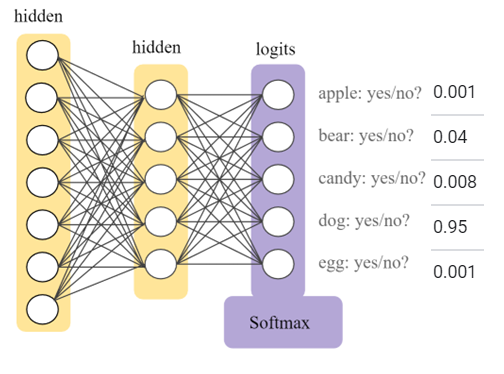
\includegraphics[width=5.25073in,height=3.89638in]{media/image6.png}

Figure 2.2.2. SoftMax-applied output layer in the neural network (purple) and probabilities for each class (right) \cite{ref17}
